
\documentclass[11pt,a4paper]{article}

\usepackage[utf8]{inputenc} 
\usepackage[T1]{fontenc} 
\usepackage{lmodern}
\usepackage{tcolorbox}

\usepackage[german]{babel}


\setlength{\parindent}{0pt}
\setlength{\parskip}{1ex plus 0.5ex minus 0.5ex}

\usepackage{amsmath} 


\usepackage{graphicx} 

\usepackage[section]{placeins}
\usepackage{booktabs}


\usepackage{hyperref}
\hypersetup{
	colorlinks,
	citecolor=red,
	filecolor=black,
	linkcolor=black,
	urlcolor=black}
\graphicspath{}

\begin{document}
	

{
	\centering 
	\large 
	Physiklabor für Anfänger*innen \\
	Ferienpraktikum im Sommersemester 2018 \\[4mm]
	\textbf{\LARGE 
		Versuch 8: Viskosität aus dem Durchströmen einer Kapillare
	} \\[3mm]
	(durchgeführt am 26.09.2018 bei Pascal Wunderlin) \\
	Ye Joon Kim, Marouan Zouari\\
	\today \\[10mm]
}
\tableofcontents
\section{Ziel des Versuchs}
Das Ziel dieses Versuchs ist es, die Viskosität von Wasser mit Kapillaren zu bestimmen. 

\begin{figure}
	\centering
	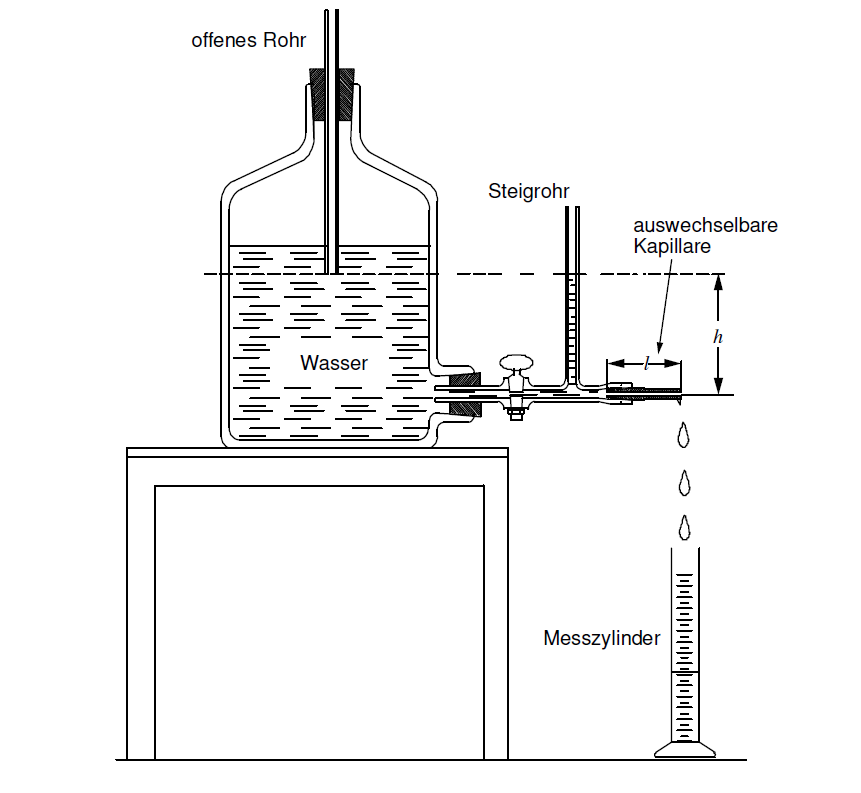
\includegraphics[scale=0.5]{pro8}
	\caption { Versuchsaufbau (,,Versuchsanleitungen'') }
\end{figure}
\section{Aufbau}
(Siehe Abbildung 1)
Für diesen Versuch wurden die folgenden Apparate benutzt: Ein großes Glas, gefüllt mit Wasser, ein T-Förmiges Rohr (inkl. Steigrohr), wodurch das Wasser fließen kann, fünf unterschiedliche Kapillare, ein Messzylinder, ein Becherglas und eine Stoppuhr. 
\section{Durchführung}

Zuerst wurden die Werte für $R^{4}/l$ von den verschiedenen Kapillaren berechnet und die Temperatur des Wassers mit einem Thermometer gemessen. 
Danach wurde eine Kapillare in das horizontale offene Rohr gesteckt und danach das Ventil  geöffnet. Dann hat das Wasser angefangen, in das Becherglas zu tropfen. Das Becherglas wurde dann schnell mit einem Messzylinder ausgetauscht und die Zeitmessung wurde angefangen, als das erste Wassertröpfchen auf den Boden des Messzylinders gefallen war. Nach einem Zeitintervall wurde das Messzylinder mit dem Becherglas wieder ausgetauscht und gleichzeitig die Zeitmessung aufgehört. Das Volumen des Wassers in dem Messzylinder und die gemessene Zeit wurden dann aufgenommen. Das wurde viermal mit unterschiedlichen Zeitintervallen wiederholt. Der gesamte Prozess wurde für unterschiedliche Kapillaren wiederholt. 
\\\
Für Genauigkeit wurde es nach dem Öffnen des Ventils einen Moment abgewartet, bis das Tropfentempo sich stabilisiert hat. Es wurde auch gecheckt, dass die Wasserhöhe in dem Steigrohr während der Zeitintervalle konstant blieb.
\\\
Am Ende des Versuchs wurde die Temperatur des Wassers nochmal gemessen.

\section{Auswertung und Fehleranalyse}
Zur Bestimmung der Viskosität wurde die folgende Formel benutzt:
\begin{equation}
	I_V = \frac{V}{t} = \frac{\pi R^4 \Delta p}{8 \eta l}
\end{equation}

Die Druckdifferenz lässt sich mit:
$$\Delta p = \rho_w hg$$
bestimmen. Deswegen bei einer Auftragung von $I_V$ gegen $\frac{R^4}{l}$ entspricht die Steigung dem Wert $\frac{ \pi \rho_w hg}{8\eta}$.
Da der Zusammenhang sich in einer Form von $I_V = a + b(\frac{R^4}{l})$ schreiben lässt , wurden die Werte für $I_V$ dann in einer Graph mit dem Programm Logger Pro gegen $\frac{R^4}{l}$ aufgetragen (Siehe Abbildung(2)). Die Werte für $a$, der Achsenabschnitt, $b$, die Steigung, und deren Unsicherheiten wurden mit einem Excel-Dokument berechnet. 

\begin{figure}    
	\centering
	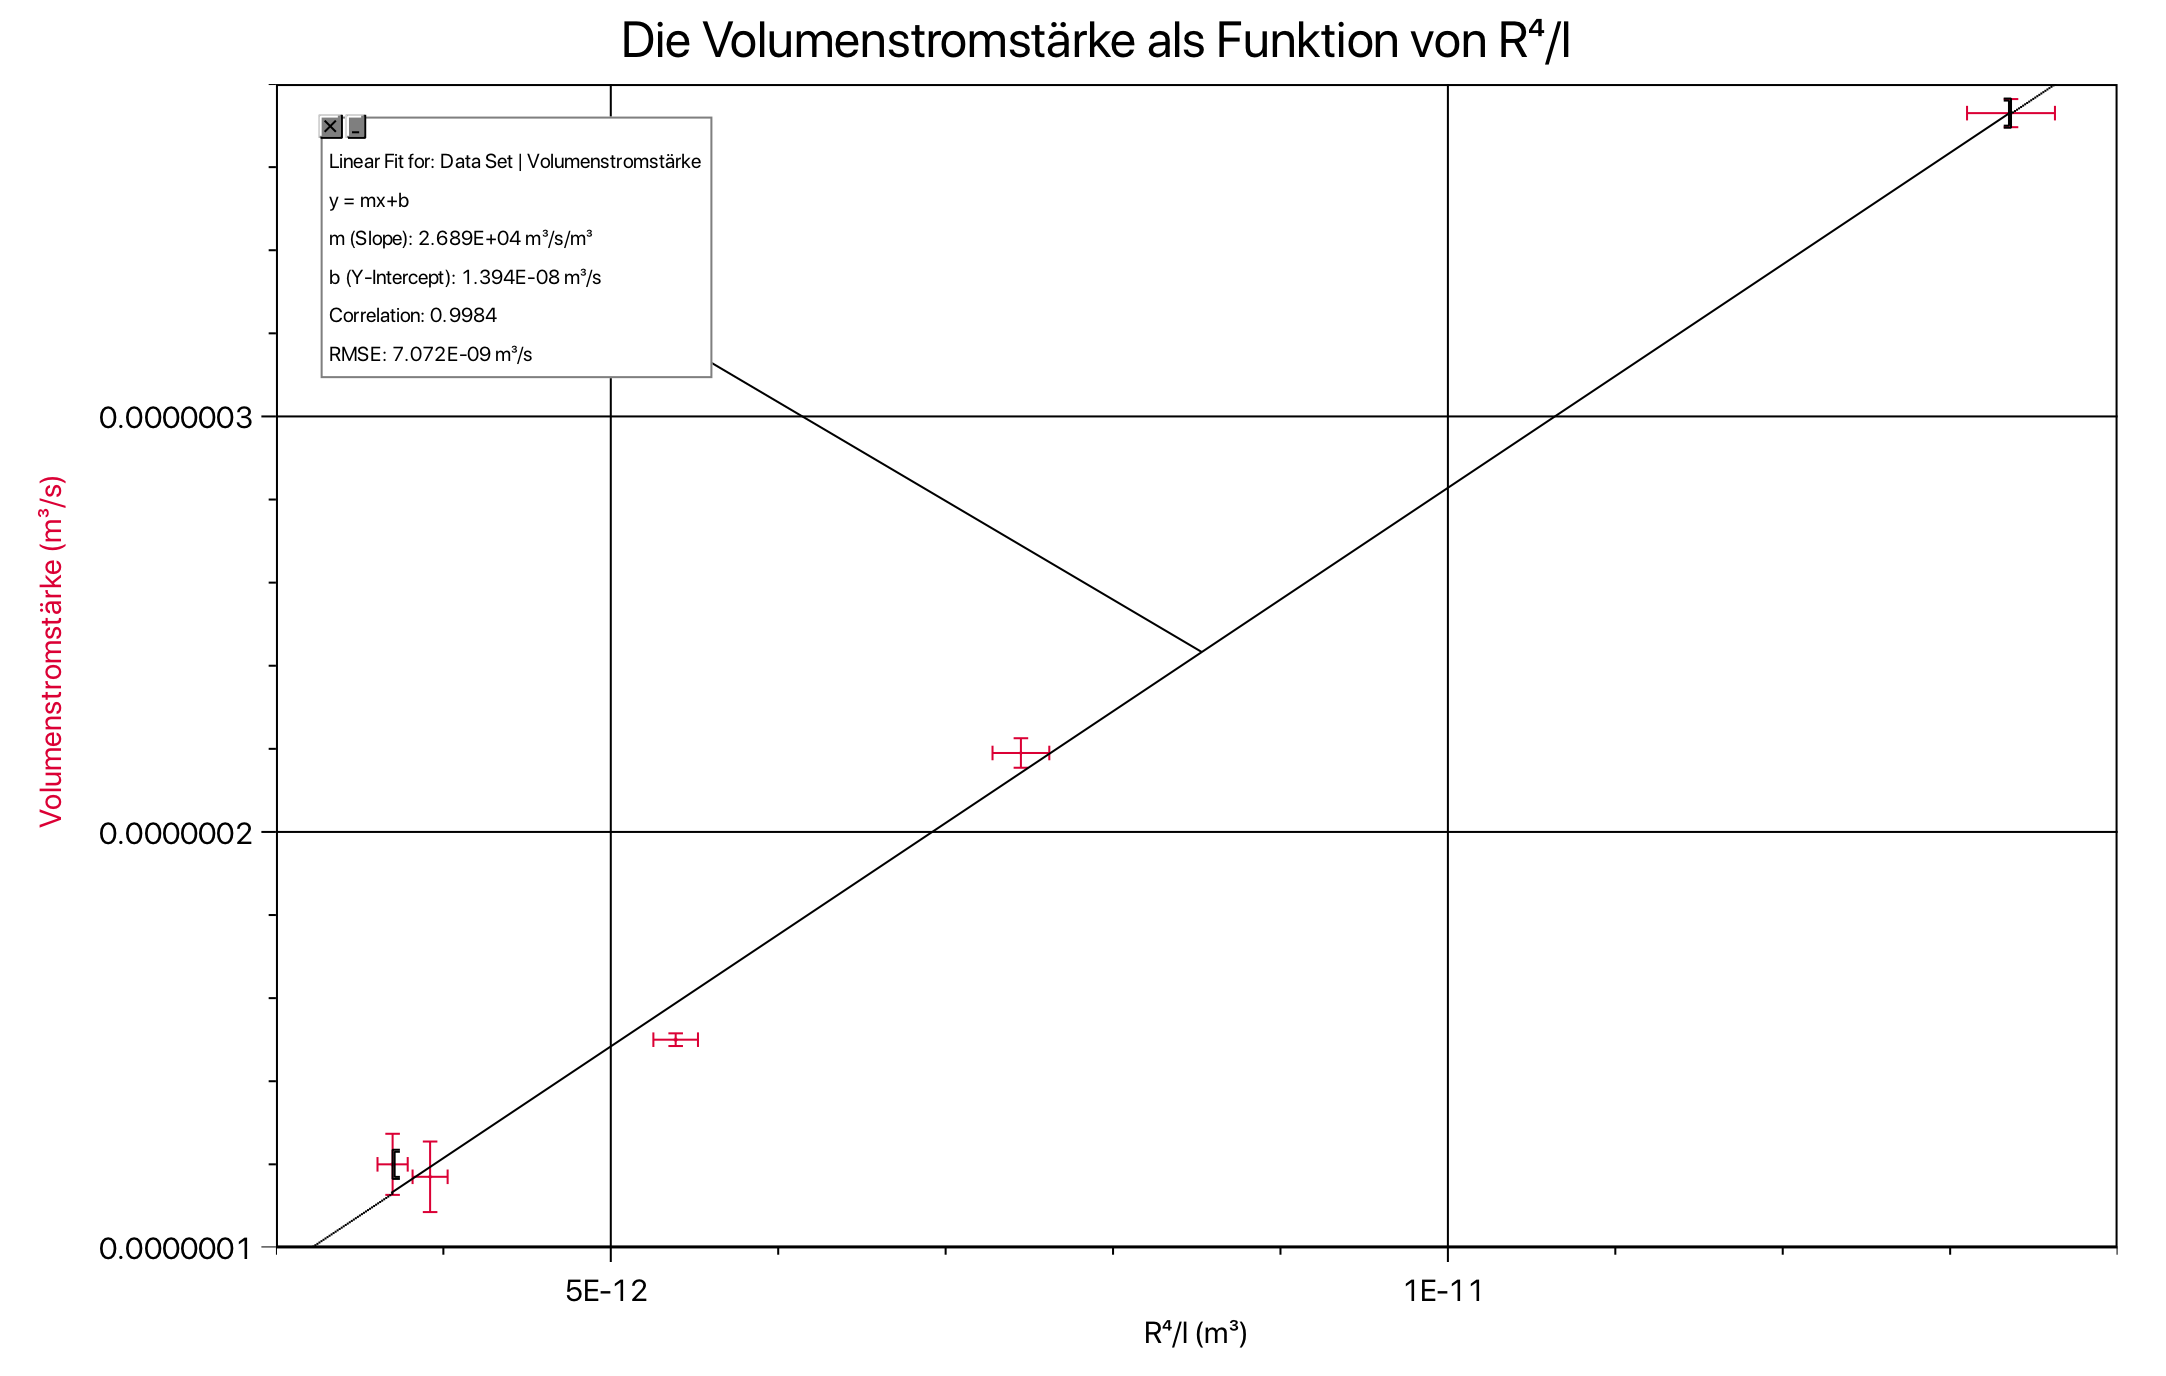
\includegraphics[width=\linewidth]{Abb2}
	\caption{Die Volumenstromstärke als Funktion von $\frac{R^4}{l}$ sowie die berechnete Ausgleichsgerade}
\end{figure}

Die lineare Regression lautet:
$$ I_V = 1,4\cdot 10^{-8} + 4,3 \cdot10^{5} (\frac{R^4}{l})$$

Mit den Unsicherheiten $u_a = 7\cdot 10^{-9}$ m$^3$/s und $u_b =1 \cdot 10^{4}$ s$^{-1}$. 

\begin{tcolorbox}[colback=white]
	\subsection{Rechenweg}
	Die Einzelnen Messwerte wurden gemittelt und in die Graph aufgetragen. Für die Unsicherheit wurde die Standardunsicherheit, oder die Standardabweichung benutzt:
	$$s_x = \sqrt{\frac{\sum_{i=1}^{n}(x_i-\bar{x})^2}{n-1}} $$
	
	Die Werte für $a$ und $b$ sowie deren Unsicherheiten lassen sich mit den folgenden Formeln bestimmen:
	$$a = \frac{
	\sum x_i^2 \sum y_i - \sum x_i \sum x_iy_i
}{
n \sum x_i^2 - (\sum x_i)^2
}$$
$$ b = \frac{
n\sum x_iy_i-\sum x_i \sum y_i
}{
n \sum x_i^2 - (\sum x_i)^2
}$$

$$u_a = s\cdot \sqrt{
\frac{
\sum x_i^2
}{
n\sum x_i^2 - (\sum x_i)^2
}}$$

$$u_b = s\cdot \sqrt{
\frac{
n
}{
n\sum x_i^2 - (\sum x_i)^2
}}$$
Mit $x = \frac{R^4}{l}$, $y = I_V$ und $s = \sqrt{
\frac{1}{n-2}\sum [y_i-(a+bx_i)]^2}$
\end{tcolorbox}

Mit der Steigung kann der Wert für $\eta$ berechnet werden. 
$$\eta = \frac{\pi \rho_w hg}{8b}$$
$$ = (1,00 \cdot 10^{-3} \pm 2\cdot10^{-5}) \textrm{Pa s} $$

\begin{tcolorbox}[colback=white]
\subsection{Rechenweg}
Zur Bestimmung der Unsicherheit von $\eta$ wurde die vereinfachte gauß'sche Fehlerfortpflanzung für Produkte und Quotienten benutzt. Deswegen ist:
$$\left\vert \frac{u_\eta}{\eta} \right \vert 
= \sqrt{(\frac{u_h}{h})^2+(\frac{u_b}{b})^2} $$
(Die Unsicherheit von $h$ wurde mit der Standardunsicherheit berechnet.)
	
\end{tcolorbox}


\section{Diskussion der Ergebnisse}
Der berechnete Wert für die Viskosität von Wasser ist:
$$\eta = (1,00 \cdot 10^{-3} \pm 2\cdot10^{-5}) \textrm{Pa s}$$

Der Literaturwert dafür beträgt:
$$\eta_\textrm{Lit} = 1,08 \cdot 10^{-3} \textrm{Pa s}$$
bei 17 $^\circ$ C (,,Viscosity of Water'').

Um zu sehen ob die gemessene und Literatur- Werte miteinander verträglich sind, wurde deren Differenz in Einheiten der Standardunsicherheit berechnet, nämlich:
$$ t_\eta = \frac{\eta_\textrm{Lit} - \eta}{u_\eta} = 4 $$
Da dieser Wert größer als 2 ist, sind das Ergebnis und der Literaturwert miteinander nicht verträglich. Das impliziert aber nicht, dass das Ergebnis unplausibel ist. Es kann auch leicht gesehen werden, dass die relative Unsicherheit 2\% ist, was auch bedeutet, dass dieses Ergebnis relativ signifikant ist. Es musste deswegen einen systematische Fehler geben, der den gemessenen Wert beeinflusst hatte. Möglicher Fehlerquellen werden in dem nächsten Abschnitt diskutiert. 


\subsection{Systematische und Statistische Fehler}
Da das Becherglas und Messzylinder von Hand bewegt werden mussten, könnte der Start der Stoppuhr und das Tropfen des Wassers auf den Boden des Messzylinders nicht immer gleichzeitig sein. Die Werte für $t$ und $V$ könnten deshalb manchmal nicht übereinstimmen. Daraus entsteht ein möglicher statistischer Fehler.

Da das System ein offenes System ist (deswegen gibt es einen Austausch von Wärme und Materie mit der Umgebung), kann die Annahme, dass die Temperatur und die Druckdifferenz konstant durch das Experiment bleiben, zu m"ogliche systematische Fehler f"uhren.

Während des Experiments hat die Temperatur des Wassers sich von $T=17^{o}C  (\pm 0,5 ^{o}C)$ zu $T=18^{o}C (\pm 0,5 ^{o}C)$ ge"andert. Wegen der starken Abhängigkeit zwischen die Temperatur und 
die Viskosität kann diese kleine Temperaturänderung zu einer Abweichung von dem Zusammenhang zwischen $\eta$ und $b$, $h$ usw. führen. Da die Viskosität  antiproportional zu der Temperatur ist, impliziert das, dass der berechnete Wert ein Bisschen niedriger als der Idealfall ist (,,Viscosity.'') . Dieses Problem lässt sich dadurch lösen, indem man die Umgebung mehr abgeschlossen macht, wie z.B die Fenster und Tür zuzumachen, damit keine signifikante Temperaturänderung entsteht. 


\section{Literatur und Bildquellen}

,,Versuchsanleitung zum Physiklabor für Anfänger*innen.'' Albert-Ludwigs-Universität Freiburg. 

,,Viscosity.'' Wikipedia. (https://en.wikipedia.org/wiki/Viscosity). 

,,Viscosity of Water.'' Anton-Paar. (https://wiki.anton-paar.com/en/water/).

\section{Anhang}
Siehe Zusatzblatt. 
	
	
	
	
	
	
	
	
	
	
\end{document}